\appendix
\section{پیوست}
\subsection{مسئله اول: مسیریابی شهرهای رومانی} \label{p1-app}
هرکدام از شهرها به ترتیب ذکر شده در شکل
\ref{p1-edited}
شماره‌گذاری شدند. در تابع شهودی مورد استفاده، فاصله واقعی هرکدام از شهرها نسبت به مقصد داده شده مورد استفاده قرار می‌گرفت که به ترتیب ذکر شده عبارتند از (عدد نوشته شده در هر سطر بیانگر فاصله واقعی آن شهر -مقدار تابع شهودی- تا مقصد است.):
\begin{latin}
	\begin{lstlisting}
710,
634,
576,
677,
408,
636,
720,
669,
561,
507,
330,
447,
388,
324,
267,
283,
387,
0,
66.6,
133,
\end{lstlisting}
\end{latin}

\begin{figure}[H]
	\centering
	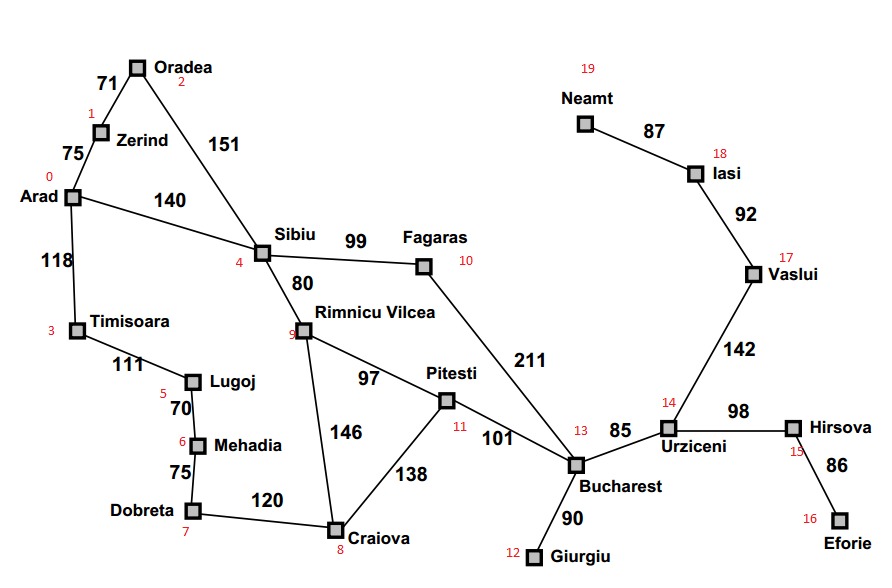
\includegraphics[width=14cm]{./Resources/p1e.png}
	\caption{شماره‌گذاری شهرهای رومانی.}
	\label{p1-edited}
\end{figure}